    \documentclass[openany]{UoYCSproject}

\protect\BEng
\protect\supervisor{Dr William Smith}
\protect\wordcount{(to-be-completed)}
\protect\includes{the title page, abstract and body of the report}
\protect\excludes{bibliographies and appendices}
\protect\abstract{This project produces a functional mobile application to visualise potential avalanche hazards along popular winter mountaineering routes within a 3D terrain reality, with a primary focus on Scottish mountains while providing excellent adaptability for other regions with appropriate data sources. Avalanche hazards were projected from a combination of professional avalanche forecasts and spatial analysis of mountain terrain models. Both the accuracy and the usability of the application were evaluated through various methods. The safety and ethical considerations on the application being put into real world use were also discussed.}

\usepackage[left=26mm,top=26mm,right=26mm,bottom=26mm]{geometry}    
\geometry{a4paper}            		
\usepackage{graphicx}					
\usepackage{amssymb}
\usepackage{url}
\usepackage[parfill]{parskip}
\usepackage{natbib}
\setlength{\headsep}{5pt}
\graphicspath{ {images/} }
\setlength{\bibsep}{3pt plus 3ex}

\title{An App for Visualisation of Avalanche Hazard}
\author{Chongyang Shi}
\date{(to-be-completed)}							
\begin{document}

{\let\cleardoublepage\clearpage 
    \maketitle
}

\chapter{Introduction}

\section{Overview of the project}

The purpose of this project is to produce a functional mobile application to visualise potential avalanche hazards along popular winter mountaineering routes within a 3D terrain reality, with a primary focus on Scottish mountains while providing excellent adaptability for other regions with appropriate data sources. 

A model for projecting localised avalanche hazards based on carefully sourced and processed avalanche forecasts \cite{sais} and terrain model data \cite{os-5} was produced by the project. The accuracy of the model has been evaluated against past avalanche records \cite[pp. 143-151]{scottish-avalanches}\cite{sais-map}. Usability and effectiveness of the application guiding the user away from hazardous locations were evaluated through experiments and test uses conducted with experienced mountaineers.

The project incorporated tools and techniques from various aspects of Computer Science, including software engineering, geographic information system (GIS) modelling, human-computer interaction, computer graphics and algorithms. Many of these tools and techniques are associated with current research in these areas.

\section{Motivations behind the application}

As a front-runner of digital avalanche forecasts, the Scottish Avalanche Information Service (SAIS) \cite{sais} have been providing frequent and reliable winter avalanche forecasts for decades in Scotland.

In addition to written observations on conditions of the snowpack and weather, a typical SAIS avalanche forecast also includes a compass ross, providing avalanche risk levels on the scale of 1 to 5 for slopes of different aspects above and below a transition threshold altitude, shown in Figure \ref{fig:mapping}. However, while this compass rose provides a comprehensive overview on avalanche risks across the forecast region, it is not straightforward to interpret, as the user will need to work out the surface aspects and altitudes along their route, and mentally infer the risk levels of different locations along their route. This is a very complex task, and prone to errors as risk levels could vary sharply between neighbouring aspects and altitudes, as shown in Figure \ref{fig:mapping}.

Therefore, the primary purpose of this project is to vastly simply this process, by generating a coloured image based on the altitude and surface aspects at each point (as determined by a terrain raster model), which is then laid on top of a computer-generated terrain model in the 3D terrain viewer. Hence the information supplied by the compass rose can be visualised in the most straightforward way, allowing the user to freely navigate the 3D model and observe the hazard levels at each location along their route. The avalanche hazard of the same area mapped in Figure \ref{fig:mapping} is visualised as shown in Figure \ref{fig:stage1bennevis}.

In later stages of the project, we also seek to improve hazard representation through constructing a custom risk model based on information from the compass rose and terrain spatial data; and to improve the functionalities of the application by adding in features such as pathfinding.

\begin{figure}[h]
		\centering
		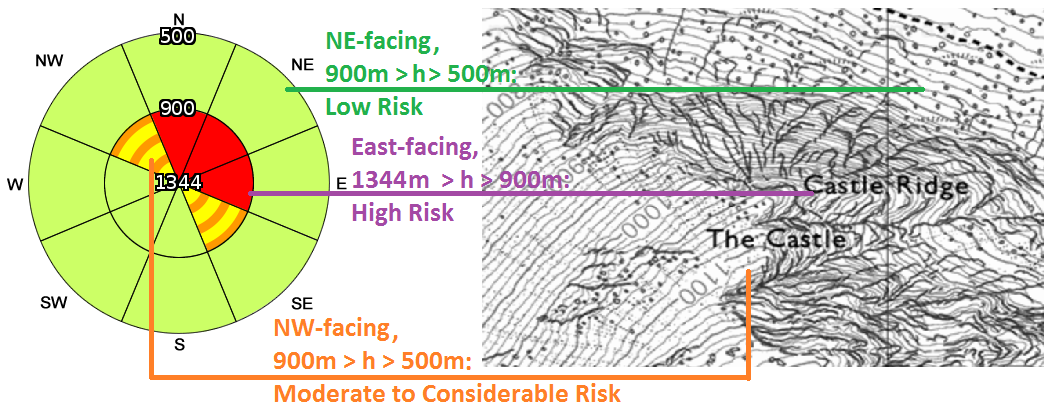
\includegraphics[scale=1]{Mapping.png}
		\caption{\label{fig:mapping} An example compass rose produced by the SAIS on January 6, 2016 for Lochaber (left), showing a steep transition of risk levels; and an example manual inference of risk levels based on the compass ross and contour lines near Ben Nevis, Lochaber (right).  \cite{sais-lochaber0106}}
\end{figure}

\begin{figure}[h]
		\centering
		\includegraphics[scale=0.25]{Stage1BenNvisDuo.png}
		\caption{\label{fig:stage1bennevis} The avalanche hazard visualisation of the same area mapped in Figure \ref{fig:mapping}, generated in the 3D terrain viewer by the initial stage product using the same avalanche forecast. The same slope is viewed from two different angles.}
\end{figure}



\section{Stages of the project}

The course of the project was divided into four development and evaluation stages, in order to effectively track and manage the workload. As the product from each stage is able to function independently of work done in other stages, risks from unforeseen difficulties encountered in research and development can be effectively mitigated. The four stages are described as followed:

\textbf{Stage 1 - Basic Functionalities:} The aim of this stage was to select an appropriate application framework and libraries to produce a basic but functional application -- a 3D terrain viewer with a hazard map overlay, the data for which would be derived solely from forecasts by the Scottish Avalanche Information Service \cite{sais}. The WebGL framework Cesium \cite{cesium} was chosen as the foundation for front-end developments, while Python was chosen to be used to develop the backend, and to interface other systems such as GIS processors with its vast range of interfacing libraries. A functional product was delivered for this stage in early November, 2016.

\textbf{Stage 2 - Improved Spatial Analysis and Evaluation:} This stage of the project expands the data source for generating the hazard map overlay by performing surface fitting and spatial analysis on the terrain model data \cite{os-5}, in order to make the hazards more localised, and to better reflect the hazard posed by unique terrain features such as concave slopes. MATLAB \cite{matlab-primer} was used to perform the computations for these purposes. Evaluations on the localised hazard map against avalanche records were also conducted at this stage, with a focus on the avalanche ``blackspots'' of Scottish mountains.

\textbf{Stage 3 - Pathfinding and Risk Calculator:} With a localised hazard map obtained in Stage 2, this stage was focused on developing a pathfinding tool for the front end application, allowing the user to plot a potential hiking path with a configurable avalanche risk level. Techniques such as A* path finding \cite{cui2011based} were utilised to develop this functionality. 

\textbf{Stage 4 - Usability Testing:} The final stage of the project focus on the human-computer interaction aspects of the application. Experienced mountaineers were consulted and invited to test use the application to provide feedbacks on usability, as well as the effectiveness of the application guiding them away from avalanches that would have occurred in real use. Some improvements were made based on the feedbacks.

\section{Considerations and statements on ethics}

The application was designed as a tool to improve winter mountaineering safety, therefore evidently the foremost consideration on ethics regarding the accuracy and robustness of avalanche hazards projected by the application. If a location with imminent avalanche threat is reported as safe by the application, a user relying on the guidance of this application could be placed in serious danger; conversely, if the application indicate avalanche warnings to users at a location where an avalanche is unlikely to occur, undue anxiety could be caused.

Due to the constraints placed on this project, it is difficult to conduct an extensive peer review process to examine the accuracy of hazard projections. And while most open source libraries utilised during the development process have been widely-used and well-tested, software errors may still occur and affect the safety assurance of the product. Furthermore, the lack of a known commercial or academic product with comparable functionalities eliminates the possibilities of cross-testing the software product.

As a result, while the application is functional and showed promise during our own evaluations, it is not considered as a product ready for real-life use -- a warning of which is displayed when a user initially accesses the application.

\section{Structure of this report}

A literature review is conducted in Chapter \ref{ch:lit-review} over existing research and developments in the various aspects of Computer Science involved in this project. The procurement and processing of both avalanche forecast and topographical data used across all stages of the project are discussed in Chapter \ref{ch:data}. Chapter \ref{ch:app-description} describes in detail the features and internal architectures of the application, as well as its development process. This is followed by Chapter \ref{ch:app-testing}, which describes the evaluation and testing conducted on the application and the quality of its data, mainly conducted during \textbf{Stage 4}. Finally, Chapter \ref{ch:conclusions} concludes the report and discusses the potential uses and future developments of the application.

\chapter{Literature Review} \label{ch:lit-review}

As an application designed to improve the usability of snow avalanche forecasts, it is necessary to first consider and evaluate past research and efforts made to understand and predict avalanches. While the term avalanche can be applied to various types of moving substances, such as rock and mud \cite[p. 1]{91097820150101}, only snow avalanches are studied by this project.

\section{Snow Avalanches}

Accumulated snow covers generally are not stable structures -- snow found in avalanches are usually 80s\% air, and cover structures gradually deform as environment temperature approaches the melting point of snow \cite[p. 16]{mcclung2006avalanche}. This instability allows avalanches to occur easily.

Snow avalanches occur when large masses of snow or ice move rapidly down a mountainside or over a precipice, often triggered from the snow cover \cite[p. 1]{91097820150101}. Avalanches can either be triggered naturally due to combinations of certain geographical \cite[p. 17]{91097820150101} and meteorological \cite[p. 23]{91097820150101} conditions, or triggered by human activities nearby \cite{schweizer2001characteristics}. Often the latter is constructive to the former when an avalanche is triggered \cite[p. 17]{mcclung2006avalanche}\cite[p .48]{scottish-avalanches}.

McClung and Schaerer \cite[p. 73]{mcclung2006avalanche} classified snow avalanches into two general types: loose snow avalanches, which usually involves surface snow and starts from a single area of the slope; and slab avalanches which are due to failures in the snow cover, resulting in blocks of snow to fall down the slope destructively. This classification is in agreement with most schemes, such as the avalanche classification by the UNESCO \cite{unesco-avalanche}, which also diversifies the classification by types of originating zones, paths and deposition zones. The diversified classification has been further improved by more recent researches \cite{91097820150101}.

Regardless of type and triggering source, avalanches are often deadly to human present nearby, especially when travelling outside areas with built-up defense \cite{91097820150101}, as it often occurs to mountaineers. During the 45 years leading up to 1999, a total of 440 fatalities from avalanche incidents were recorded in the United States \cite{PAGE1999146}; while in the UK, avalanches in Scottish mountains alone claimed at least 73 lives during a similar time period \cite{scottish-avalanches}. 

With a prosperous winter sport industry bringing millions to mountains and resorts every year\cite{hudson2003sport}, accurate forecasting of avalanches is becoming increasingly critical. 

\section{Avalanche Forecasting}

Avalanche forecasting is defined as predictions of current and future snow instability in space and time relative to a given triggering level for avalanche initiation \cite[p. 131]{McClung2002}. When applied, the main concerns of such predictions are of risk to humans or property. 

A conventionally approach to avalanche forecasting involves extensive field observations and testings of the snow cover by experienced forecasters and mountain guides, cross-referencing of historic meteorological and avalanche records, and utilisation of statistical and information theory methods on data collected to reduce decision uncertainties, as summarised by LaChapelle \cite{lachapelle1980fundamental} in 1980. This is still very similar to the approach the Scottish Avalanche Information Service (SAIS) today \cite[p. 5]{sais2014-15}. In this style of approach, final decisions on hazard levels are heavily reliant on the experience and judgement of the experienced forecasters. LaChapelle noted \cite[p. 76]{lachapelle1980fundamental} that while inaccuracies do occur in forecasters' decisions, complete failures are rare. McClung \cite{mcclung2006avalanche} further analysed the influence of human perceptions in avalanche forecasting, and gave a formalised decision-making process to eliminate biases and improve accuracy.

While human decision-making still plays a dominant role in forecasting avalanche hazard levels, computational models have been developed to improve data analysis and to provide supplementary opinions through machine learning methods, backed by a vast increase in accessible computing power, as McClung \cite{McClung1994} has explored as early as in 1994. Numerous models have since been developed, with computations performed on different data sources. 

\textit{SNOWPACK}, a snow profile comparison method was first published by Lehning \textit{et al.} \cite{Lehning2001253} in 2001. The method attempts to establish a numerical profile of snow cover conditions based on various measured properties of the cover, such as the size and type of snow grains, temperature and density of the environments. A agreement score could then be established by comparing the numerical profile with an observed profile in the field, with high agreement scores reached by the experiments, indicating that the numerical profile would be suitable for use in avalanche forecasts. 

However, attempts to apply SNOWPACK to other regions with different snow conditions have identified weaknesses in the assumptions made in the model, which was originally developed for the Swiss Alps. A notable attempt was made by Hirashima \textit{et al.} \cite{Hirashima2008191} from 2005 to 2006 in Tsunan, Japan. While numerical profiles computed were in reasonable agreement with the observed snow profiles in Tsunan, it was found that the stability index estimators embedded in the model was not suitable for the shear strength Japanese snow, and an alternative method for calculating the index had to be adopted. This suggests adaptation of \textit{SNOWPACK} to a new region may require appropriate changes to the model based on local snow conditions.

While SNOWPACK was developed as a specialised method for analysis of snow covers, more generalised models such as the Nearest Neighbours (NN) method have also been developed. The NN model was initially developed by Buser \cite{buser1983avalanche} in 1983, which has been improved and supplemented by various studies, such as Purves \textit{et al.} in 2003, and Singh and Ganju \cite{Singh2004105} \cite{Singh201533} since 2004. The NN method applies a machine learning approach on historic avalanche and meteorological records, as well as spatial data to estimate the likelihood of an avalanche under the current conditions of a location. As the NN method has difficulties with high dimensional data, an alternative method based on Support Vector Machines (SVMs) have been proposed and developed \cite{Lehning2001253} \cite{pozdnoukhov2011spatio}.

\begin{figure}[h]
		\centering
		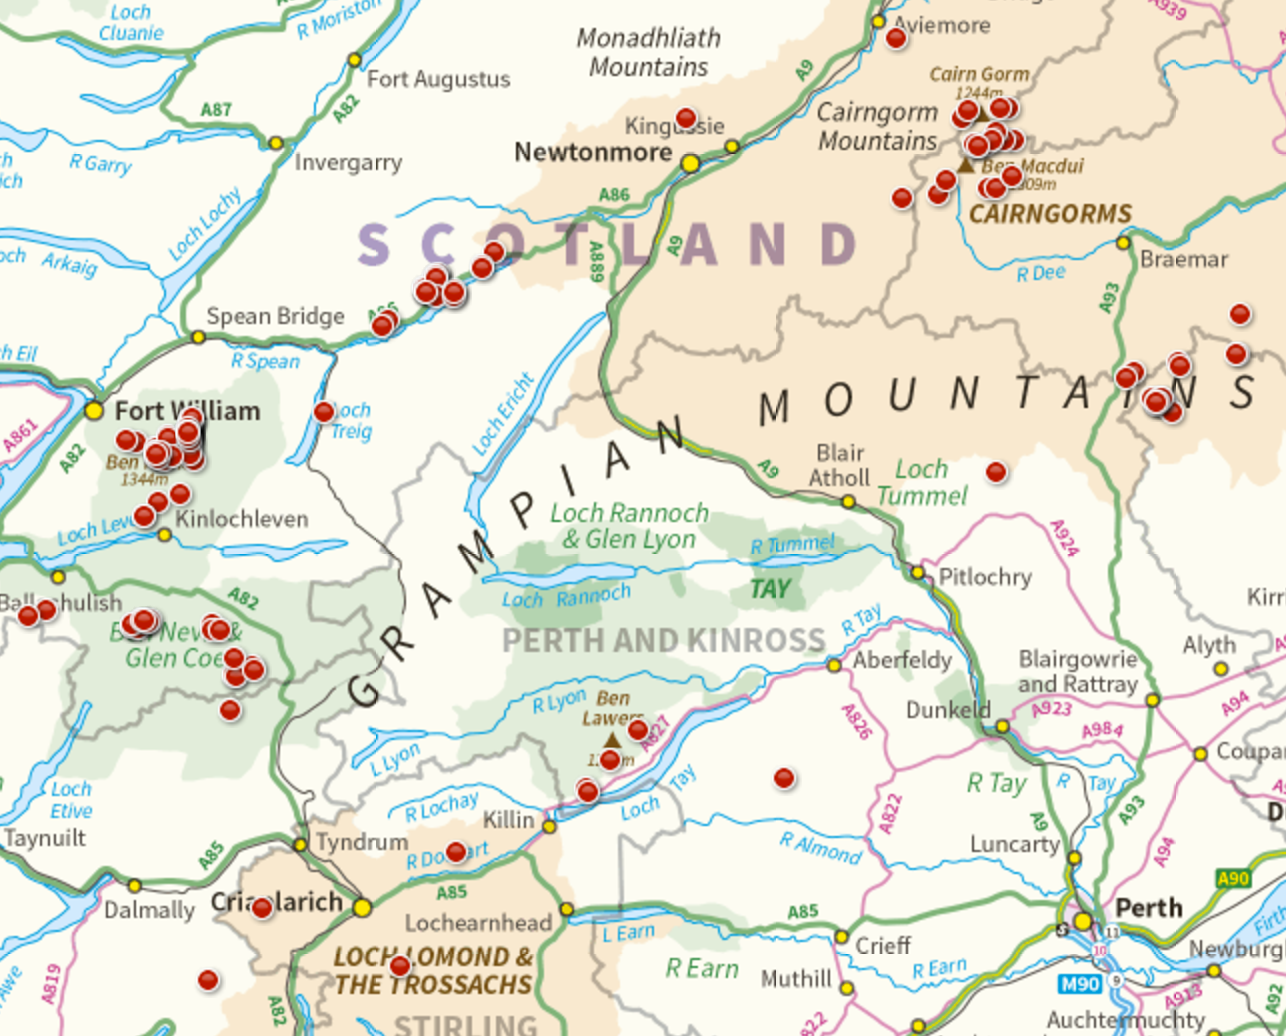
\includegraphics[scale=0.4]{ScotAvalanches1516.png}
		\caption{\label{fig:scotava1516} User-reported avalanches in the Cairngorms and the Glencoe regions during winter sports season of 2015-2016, generated by the SAIS.\cite{sais-map}}
\end{figure}

The most notable application of the NN method is by the SAIS. Avalanche forecasts from the SAIS partially dependent on the NN method achieved a weighted accuracy of between 71\% and 82\% on visible winter days between 1988 and 2002 \cite[p. 351] {Purves2003343}. With up to 205 avalanches reported by mountaineers during the winter season of 2015-2016 \cite{sais} (as partly shown in Figure \ref{fig:scotava1516}), the SAIS plays a very significant role in saving lives from avalanches. Data from SAIS forecasts would also be a critical component in data sourcing and hazard modelling during this project.

In addition to analysis of snow and terrain conditions and past avalanche records, studies of vegetations in mountainous areas can also provide important information on recurrence of avalanches. Christophe \textit{et al.} \cite{Christophe2010107} developed a model based on observation of tree-rings. As avalanches affect the growth of trees and other vegetations on the mountain slopes, growth condition of trees would provide useful insight into the magnitude and frequency of past avalanches in the area. One downside of the model is its unsuitableness for direct use in temporal avalanche forecasts, as the formation of general vegetation conditions requires a long period of time. However, for the purpose of this project this model could potentially be used for establishing a static risk level for each point in the terrain, to be included in the overall risk model.
 
\chapter{Procurement and Processing of Data} \label{ch:data}

\chapter{Description of the Application} \label{ch:app-description}

\chapter{Evaluation and Testing of the Application} \label{ch:app-testing}

\chapter{Conclusions} \label{ch:conclusions}

\small{\bibliography{project}}
\end{document}  